\documentclass{article}

\usepackage{graphicx}
\usepackage{tikz}
\usepackage{tikzsymbols}
\usetikzlibrary{calc,patterns,shapes.geometric}
\pagestyle{empty}
\usepackage[margin=0pt]{geometry}
\geometry{papersize={14in,12in}}

\def\centerarc[#1](#2)(#3:#4:#5){\draw[#1] ($(#2)+({#5*cos(#3)},{#5*sin(#3)})$) arc (#3:#4:#5);}

\begin{document}
	\begin{figure}
		\centering
		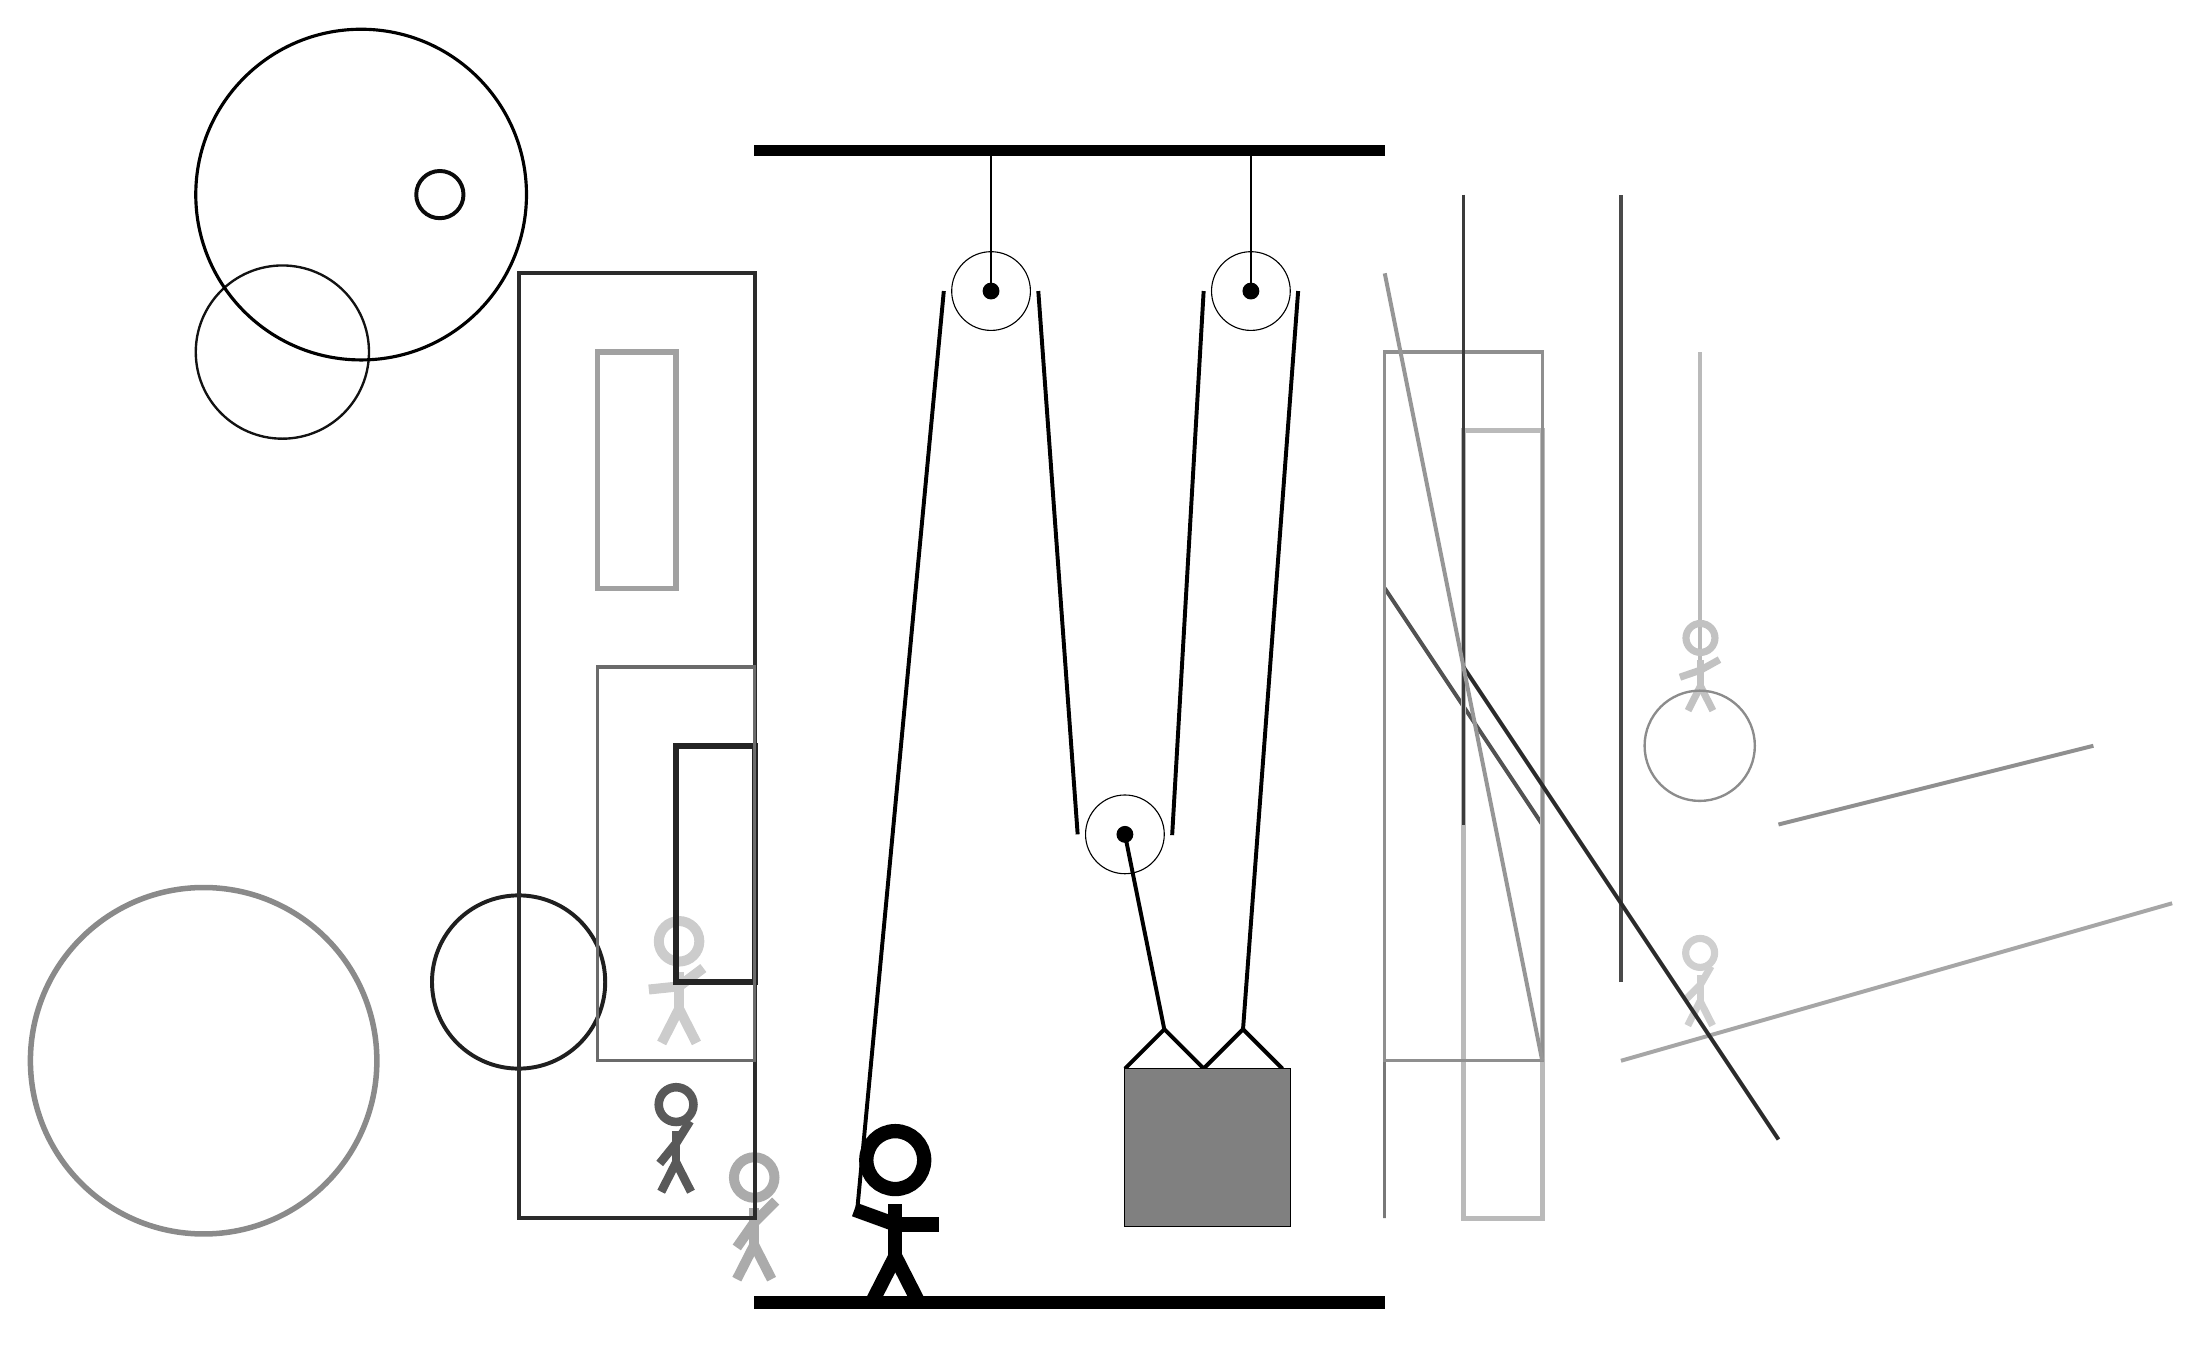
\begin{tikzpicture}
			%%%%% START %%%%%
			
			\draw[fill=black] (-2, 11.5) rectangle (6, 11.625);
			
			\draw (1, 9.775) circle (0.5);
			\draw[fill=black] (1, 9.775) circle (0.1);
			\draw[thick] (1, 9.775) -- (1, 11.5);
			
			\draw (4.3, 9.775) circle (0.5);
			\draw[fill=black] (4.3, 9.775) circle (0.1);
			\draw[thick] (4.3, 9.775) -- (4.3, 11.5);
			
			\draw (2.7, 2.875) circle (0.5);
			\draw[fill=black] (2.7, 2.875) circle (0.1);
			
			\draw[line width=0.5mm]  (2.7, -0.1) -- (3.2, 0.4) -- (3.7, -0.1) -- (4.2, 0.4) -- (4.7, -0.1);
			\draw[fill=black!50] (2.7, -0.1) rectangle (4.8, -2.1);
			
			\draw[line width=0.5mm](-0.7, -1.9) -- (0.4, 9.775);
			\centerarc[line width=0.5mm](1, 9.775)(0:180:0.6);
			\draw[line width=0.5mm](1.6, 9.775) -- (2.1, 2.875);
			\centerarc[line width=0.5mm](2.7, 2.875)(180:370:0.6);
			\draw[line width=0.5mm] (3.3, 2.865) -- (3.7, 9.775);
			\centerarc[line width=0.5mm](4.3, 9.775)(0:180:0.6);
			\draw[line width=0.5mm](4.2, 0.4) -- (4.9, 9.775);
			\draw[line width=0.5mm] (3.2, 0.4) -- (2.7, 2.875);
			
			\draw[line width=0.5mm, color=black!35](9, 0) -- (16, 2);
			
			\draw [line width=0.3mm, color=black!93](-8, 9) circle (1.1);
			\draw [line width=0.4mm, color=black!100](-7, 11) circle (2.1);
			\draw [line width=0.5mm, color=black!88](-5, 1) circle (1.1);
			\node[line width=0.5mm, color=black!65] at (-3, -1) {\Strichmaxerl[6][51][58]};
			
			\draw[line width=0.5mm, color=black!68](8, 3) -- (6, 6);
			\draw[line width=0.4mm, color=black!53] (6, -2) rectangle (6, 8);
			\draw[line width=0.5mm, color=black!71](9, 1) -- (9, 11);
			\draw[line width=0.6mm, color=black!27] (7, -2) rectangle (8, 8);
			
			\draw[line width=0.4mm, color=black!44] (6, 0) rectangle (8, 9);
			\draw[line width=0.5mm, color=black!27](10, 5) -- (10, 9);
			\draw [line width=0.7mm, color=black!46](-9, 0) circle (2.2);
			\node[line width=0.6mm, color=black!20] at (-3, 1) {\Strichmaxerl[7][6][37]};
			
			\node[line width=0.4mm, color=black!24] at (10, 5) {\Strichmaxerl[5][19][29]};
			\draw[line width=0.5mm, color=black!77](7, 11) -- (7, 3);
			\node[line width=0.7mm, color=black!19] at (10, 1) {\Strichmaxerl[5][45][60]};
			\draw[line width=0.5mm, color=black!83](11, -1) -- (7, 5);
			
			\draw[line width=0.5mm, color=black!44](11, 3) -- (15, 4);
			\node[line width=0.6mm, color=black!33] at (-2, -2) {\Strichmaxerl[7][55][45]};
			\draw [line width=0.3mm, color=black!45](10, 4) circle (0.7);
			\draw[line width=0.7mm, color=black!37] (-3, 9) rectangle (-4, 6);
			
			\draw[line width=0.5mm, color=black!83] (-2, -2) rectangle (-5, 10);
			\draw[line width=0.7mm, color=black!86] (-2, 4) rectangle (-3, 1);
			\draw[line width=0.5mm, color=black!41](8, 0) -- (6, 10);
			\draw[line width=0.4mm, color=black!58] (-4, 5) rectangle (-2, 0);
			
			\draw [line width=0.5mm, color=black!96](-6, 11) circle (0.3);
			
			
			\node at (-0.2, -2) {\Strichmaxerl[10][-20][0]};
			
			\draw[fill=black] (-2, -3) rectangle (6, -3.15);
			
			%%%%% END %%%%%
		\end{tikzpicture}
	\end{figure}	
\end{document}